\documentclass [11pt]{article}
\usepackage {amssymb,amsmath,graphicx,enumitem}

\usepackage[tmargin=0.7in,bmargin=0.2in,hmargin=1in]{geometry}

\setlength{\parskip}{.1in}  
\setlength{\parindent}{0.0in}  

\usepackage{enumitem}
\setlist{topsep=-.5em,itemsep=-0.25em,leftmargin=0.4cm}
\pagestyle{plain} 

\begin{document}
\centerline{\textbf{A Bifurcation Analysis using Rpplane}}

The Rosenzweig-MacArthur model is a simple model for
predator-prey population dynamics, somewhat plausible and the starting point for more realistic models. The state
variables are $n_1$ (abundance of prey) and $n_2$ (abundance of predators):   
\begin{equation}
\begin{gathered}
  \frac{dn_1}{dt} = r_1 n_1 (1 - n_1 /K ) - \frac{a_1 n_1 n_2}{B + n_1} \hfill \\ 
  \frac{dn_2}{dt} = \frac{a_2 n_1 n_2}{B + n_1} - d_2 n_2 \hfill  \\ 
\end{gathered}
\label{RosMacModel} 
\end{equation}
All parameters are positive. The first term in $dn_1/dt$ is how the prey population grows when predators are absent,  
including births and deaths. $\frac{a_1 n_1 n_2}{B+n_1}$ is the rate of prey-predator encounters that result 
in a prey being killed and eaten. The numerator is like the $\beta SI$ infection rate
in the SIR model, and the denominator represents 
the reduction in encounter rate because predators can't hunt and eat at the same time. 
In $dn_2/dt$, the first term is conversion of food to babies, and the second is predator mortality. 

The exercise is: use Rpplane to construct a bifurcation diagram for this model as a function of $K$, for other
parameters having values $r_1=d_2=1, a_1 = a_2 = 2, B=200$. Note for any parameter values, there are two equilibria: 
\begin{itemize}
\item $n_1 = n_2 = 0$ (nobody at all) 
\item $n_1 = K, n_2 = 0$ (prey only) 
\end{itemize} 
and for some parameter values there is also a \emph{coexistence equilibrium} 
where prey and predators coexist: $n_1 >0, n_2 >0$. The value of $K$ 
affects the existence of the coexistence equilibrium, and the stability of each equilibrium. 

The script \texttt{Rpplane-RosMac.R} starts you off at $K=100$. As you will see, $K=100$ is a low value and
nothing will change by making it even smaller. What happens as $K$ increases? Fill in a diagram like the one below, 
indicating when each equilibrium is stable (solid) vs. unstable (dashed), and anything else of interest. The dashed
line represents the prey-only equilibrium $n_1=K, n_2=0$, but don't believe what it says about stability. 

Here's a hint: The coexistence equilibrium (when it exists) is a point on the predator nullcline, in the region where $n_2 > 0$. 
What is the predator nullcline, and what does that say about the value of the prey abundance $\bar{n}_1$ at 
the coexistence equilibrium (using pencil and paper)? 

\centerline{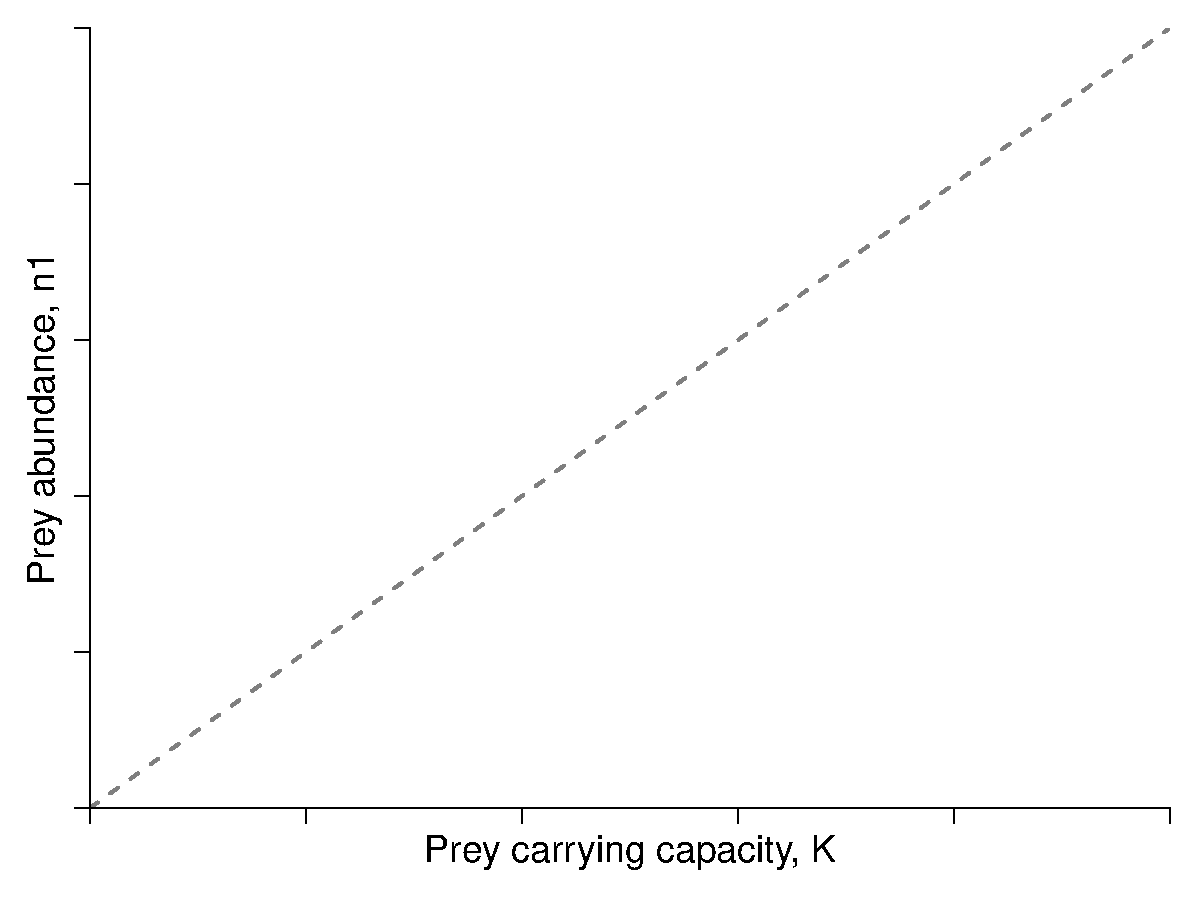
\includegraphics[width=0.6\textwidth]{RMbifur.pdf}}






\end{document}
